% Created by tikzDevice version 0.10.1 on 2016-06-15 07:22:32
% !TEX encoding = UTF-8 Unicode
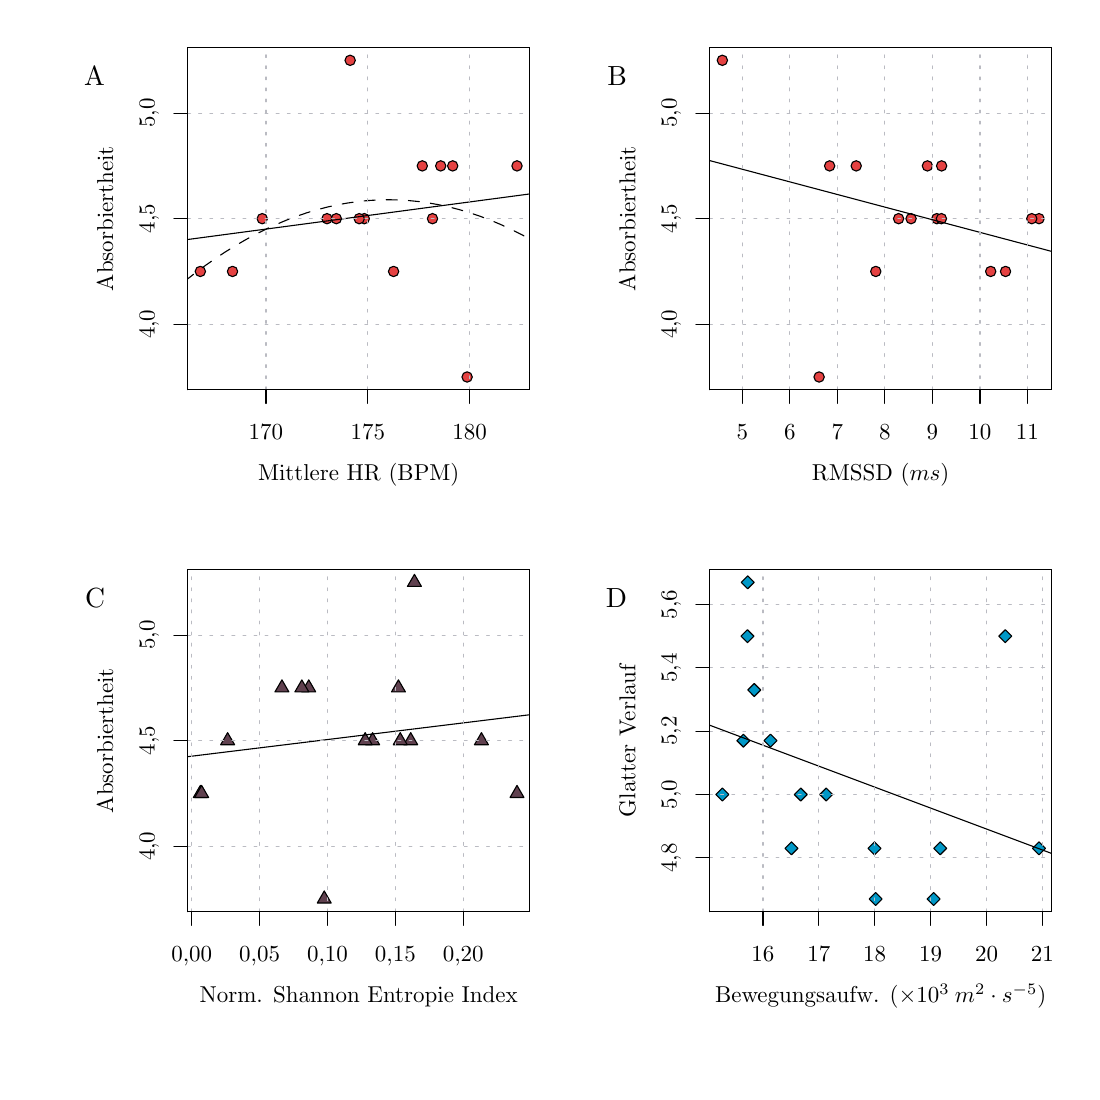
\begin{tikzpicture}[x=1pt,y=1pt]
\definecolor{fillColor}{RGB}{255,255,255}
\path[use as bounding box,fill=fillColor,fill opacity=0.00] (0,0) rectangle (377.25,377.25);
\begin{scope}
\path[clip] ( 57.82,246.44) rectangle (181.40,370.02);
\definecolor{drawColor}{RGB}{0,0,0}
\definecolor{fillColor}{RGB}{229,66,66}

\path[draw=drawColor,line width= 0.4pt,line join=round,line cap=round,fill=fillColor] ( 62.39,289.16) circle (  1.87);

\path[draw=drawColor,line width= 0.4pt,line join=round,line cap=round,fill=fillColor] ( 84.76,308.23) circle (  1.87);

\path[draw=drawColor,line width= 0.4pt,line join=round,line cap=round,fill=fillColor] ( 74.02,289.16) circle (  1.87);

\path[draw=drawColor,line width= 0.4pt,line join=round,line cap=round,fill=fillColor] (121.64,308.23) circle (  1.87);

\path[draw=drawColor,line width= 0.4pt,line join=round,line cap=round,fill=fillColor] (146.28,308.23) circle (  1.87);

\path[draw=drawColor,line width= 0.4pt,line join=round,line cap=round,fill=fillColor] (132.22,289.16) circle (  1.87);

\path[draw=drawColor,line width= 0.4pt,line join=round,line cap=round,fill=fillColor] (119.80,308.23) circle (  1.87);

\path[draw=drawColor,line width= 0.4pt,line join=round,line cap=round,fill=fillColor] (142.59,327.30) circle (  1.87);

\path[draw=drawColor,line width= 0.4pt,line join=round,line cap=round,fill=fillColor] (176.82,327.30) circle (  1.87);

\path[draw=drawColor,line width= 0.4pt,line join=round,line cap=round,fill=fillColor] (108.16,308.23) circle (  1.87);

\path[draw=drawColor,line width= 0.4pt,line join=round,line cap=round,fill=fillColor] (149.25,327.30) circle (  1.87);

\path[draw=drawColor,line width= 0.4pt,line join=round,line cap=round,fill=fillColor] (153.58,327.30) circle (  1.87);

\path[draw=drawColor,line width= 0.4pt,line join=round,line cap=round,fill=fillColor] (111.53,308.23) circle (  1.87);

\path[draw=drawColor,line width= 0.4pt,line join=round,line cap=round,fill=fillColor] (116.53,365.45) circle (  1.87);

\path[draw=drawColor,line width= 0.4pt,line join=round,line cap=round,fill=fillColor] (158.79,251.02) circle (  1.87);
\end{scope}
\begin{scope}
\path[clip] (  0.00,  0.00) rectangle (377.25,377.25);
\definecolor{drawColor}{RGB}{0,0,0}

\path[draw=drawColor,line width= 0.4pt,line join=round,line cap=round] ( 86.11,246.44) -- (159.71,246.44);

\path[draw=drawColor,line width= 0.4pt,line join=round,line cap=round] ( 86.11,246.44) -- ( 86.11,241.46);

\path[draw=drawColor,line width= 0.4pt,line join=round,line cap=round] (122.91,246.44) -- (122.91,241.46);

\path[draw=drawColor,line width= 0.4pt,line join=round,line cap=round] (159.71,246.44) -- (159.71,241.46);

\node[text=drawColor,anchor=base,inner sep=0pt, outer sep=0pt, scale=  0.83] at ( 86.11,228.51) {170};

\node[text=drawColor,anchor=base,inner sep=0pt, outer sep=0pt, scale=  0.83] at (122.91,228.51) {175};

\node[text=drawColor,anchor=base,inner sep=0pt, outer sep=0pt, scale=  0.83] at (159.71,228.51) {180};

\path[draw=drawColor,line width= 0.4pt,line join=round,line cap=round] ( 57.82,270.09) -- ( 57.82,346.37);

\path[draw=drawColor,line width= 0.4pt,line join=round,line cap=round] ( 57.82,270.09) -- ( 52.84,270.09);

\path[draw=drawColor,line width= 0.4pt,line join=round,line cap=round] ( 57.82,308.23) -- ( 52.84,308.23);

\path[draw=drawColor,line width= 0.4pt,line join=round,line cap=round] ( 57.82,346.37) -- ( 52.84,346.37);

\node[text=drawColor,rotate= 90.00,anchor=base,inner sep=0pt, outer sep=0pt, scale=  0.83] at ( 45.86,270.09) {4,0};

\node[text=drawColor,rotate= 90.00,anchor=base,inner sep=0pt, outer sep=0pt, scale=  0.83] at ( 45.86,308.23) {4,5};

\node[text=drawColor,rotate= 90.00,anchor=base,inner sep=0pt, outer sep=0pt, scale=  0.83] at ( 45.86,346.37) {5,0};

\path[draw=drawColor,line width= 0.4pt,line join=round,line cap=round] ( 57.82,246.44) --
	(181.40,246.44) --
	(181.40,370.02) --
	( 57.82,370.02) --
	( 57.82,246.44);
\end{scope}
\begin{scope}
\path[clip] (  0.00,188.62) rectangle (188.62,377.25);
\definecolor{drawColor}{RGB}{0,0,0}

\node[text=drawColor,anchor=base,inner sep=0pt, outer sep=0pt, scale=  0.83] at (119.61,213.57) {Mittlere HR (BPM)};

\node[text=drawColor,rotate= 90.00,anchor=base,inner sep=0pt, outer sep=0pt, scale=  0.83] at ( 30.92,308.23) {Absorbiertheit};
\end{scope}
\begin{scope}
\path[clip] ( 57.82,246.44) rectangle (181.40,370.02);
\definecolor{drawColor}{RGB}{0,0,0}

\path[draw=drawColor,line width= 0.4pt,line join=round,line cap=round] ( 57.82,300.70) -- (181.40,317.16);

\path[draw=drawColor,line width= 0.4pt,dash pattern=on 4pt off 4pt ,line join=round,line cap=round] ( 12.51,239.64) --
	( 16.19,244.27) --
	( 19.87,248.76) --
	( 23.55,253.11) --
	( 27.23,257.31) --
	( 30.91,261.35) --
	( 34.59,265.26) --
	( 38.27,269.01) --
	( 41.95,272.62) --
	( 45.63,276.08) --
	( 49.31,279.39) --
	( 52.99,282.56) --
	( 56.67,285.58) --
	( 60.35,288.45) --
	( 64.03,291.18) --
	( 67.71,293.76) --
	( 71.39,296.19) --
	( 75.07,298.47) --
	( 78.75,300.61) --
	( 82.43,302.60) --
	( 86.11,304.44) --
	( 89.79,306.13) --
	( 93.47,307.68) --
	( 97.15,309.08) --
	(100.83,310.34) --
	(104.51,311.44) --
	(108.19,312.40) --
	(111.87,313.21) --
	(115.55,313.88) --
	(119.23,314.40) --
	(122.91,314.77) --
	(126.59,314.99) --
	(130.27,315.07) --
	(133.95,315.00) --
	(137.63,314.78) --
	(141.31,314.41) --
	(144.99,313.90) --
	(148.67,313.24) --
	(152.35,312.44) --
	(156.03,311.48) --
	(159.71,310.38) --
	(163.39,309.13) --
	(167.07,307.74) --
	(170.75,306.20) --
	(174.43,304.51) --
	(178.11,302.67) --
	(181.79,300.69) --
	(185.47,298.56) --
	(189.15,296.28) --
	(192.83,293.85) --
	(196.51,291.28) --
	(200.19,288.56) --
	(203.87,285.70) --
	(207.55,282.68) --
	(211.23,279.52) --
	(214.91,276.21) --
	(218.59,272.76) --
	(222.27,269.16) --
	(225.95,265.41) --
	(229.63,261.51) --
	(233.31,257.47);
\definecolor{drawColor}{RGB}{186,187,194}

\path[draw=drawColor,line width= 0.4pt,dash pattern=on 1pt off 3pt ,line join=round,line cap=round] ( 86.11,246.44) -- ( 86.11,370.02);

\path[draw=drawColor,line width= 0.4pt,dash pattern=on 1pt off 3pt ,line join=round,line cap=round] (122.91,246.44) -- (122.91,370.02);

\path[draw=drawColor,line width= 0.4pt,dash pattern=on 1pt off 3pt ,line join=round,line cap=round] (159.71,246.44) -- (159.71,370.02);

\path[draw=drawColor,line width= 0.4pt,dash pattern=on 1pt off 3pt ,line join=round,line cap=round] ( 57.82,270.09) -- (181.40,270.09);

\path[draw=drawColor,line width= 0.4pt,dash pattern=on 1pt off 3pt ,line join=round,line cap=round] ( 57.82,308.23) -- (181.40,308.23);

\path[draw=drawColor,line width= 0.4pt,dash pattern=on 1pt off 3pt ,line join=round,line cap=round] ( 57.82,346.37) -- (181.40,346.37);
\end{scope}
\begin{scope}
\path[clip] (  0.00,  0.00) rectangle (377.25,377.25);
\definecolor{drawColor}{RGB}{0,0,0}

\path[draw=drawColor,line width= 0.4pt,line join=round,line cap=round] ( 57.82,246.44) --
	(181.40,246.44) --
	(181.40,370.02) --
	( 57.82,370.02) --
	( 57.82,246.44);

\node[text=drawColor,anchor=base east,inner sep=0pt, outer sep=0pt, scale=  1.00] at ( 27.94,356.44) {A};
\end{scope}
\begin{scope}
\path[clip] (246.44,246.44) rectangle (370.02,370.02);
\definecolor{drawColor}{RGB}{0,0,0}
\definecolor{fillColor}{RGB}{229,66,66}

\path[draw=drawColor,line width= 0.4pt,line join=round,line cap=round,fill=fillColor] (347.99,289.16) circle (  1.87);

\path[draw=drawColor,line width= 0.4pt,line join=round,line cap=round,fill=fillColor] (328.51,308.23) circle (  1.87);

\path[draw=drawColor,line width= 0.4pt,line join=round,line cap=round,fill=fillColor] (306.46,289.16) circle (  1.87);

\path[draw=drawColor,line width= 0.4pt,line join=round,line cap=round,fill=fillColor] (365.45,308.23) circle (  1.87);

\path[draw=drawColor,line width= 0.4pt,line join=round,line cap=round,fill=fillColor] (362.83,308.23) circle (  1.87);

\path[draw=drawColor,line width= 0.4pt,line join=round,line cap=round,fill=fillColor] (353.35,289.16) circle (  1.87);

\path[draw=drawColor,line width= 0.4pt,line join=round,line cap=round,fill=fillColor] (330.17,308.23) circle (  1.87);

\path[draw=drawColor,line width= 0.4pt,line join=round,line cap=round,fill=fillColor] (325.12,327.30) circle (  1.87);

\path[draw=drawColor,line width= 0.4pt,line join=round,line cap=round,fill=fillColor] (330.25,327.30) circle (  1.87);

\path[draw=drawColor,line width= 0.4pt,line join=round,line cap=round,fill=fillColor] (314.70,308.23) circle (  1.87);

\path[draw=drawColor,line width= 0.4pt,line join=round,line cap=round,fill=fillColor] (299.39,327.30) circle (  1.87);

\path[draw=drawColor,line width= 0.4pt,line join=round,line cap=round,fill=fillColor] (289.79,327.30) circle (  1.87);

\path[draw=drawColor,line width= 0.4pt,line join=round,line cap=round,fill=fillColor] (319.21,308.23) circle (  1.87);

\path[draw=drawColor,line width= 0.4pt,line join=round,line cap=round,fill=fillColor] (251.02,365.45) circle (  1.87);

\path[draw=drawColor,line width= 0.4pt,line join=round,line cap=round,fill=fillColor] (285.98,251.02) circle (  1.87);
\end{scope}
\begin{scope}
\path[clip] (  0.00,  0.00) rectangle (377.25,377.25);
\definecolor{drawColor}{RGB}{0,0,0}

\path[draw=drawColor,line width= 0.4pt,line join=round,line cap=round] (258.28,246.44) -- (361.26,246.44);

\path[draw=drawColor,line width= 0.4pt,line join=round,line cap=round] (258.28,246.44) -- (258.28,241.46);

\path[draw=drawColor,line width= 0.4pt,line join=round,line cap=round] (275.44,246.44) -- (275.44,241.46);

\path[draw=drawColor,line width= 0.4pt,line join=round,line cap=round] (292.61,246.44) -- (292.61,241.46);

\path[draw=drawColor,line width= 0.4pt,line join=round,line cap=round] (309.77,246.44) -- (309.77,241.46);

\path[draw=drawColor,line width= 0.4pt,line join=round,line cap=round] (326.93,246.44) -- (326.93,241.46);

\path[draw=drawColor,line width= 0.4pt,line join=round,line cap=round] (344.10,246.44) -- (344.10,241.46);

\path[draw=drawColor,line width= 0.4pt,line join=round,line cap=round] (361.26,246.44) -- (361.26,241.46);

\node[text=drawColor,anchor=base,inner sep=0pt, outer sep=0pt, scale=  0.83] at (258.28,228.51) {5};

\node[text=drawColor,anchor=base,inner sep=0pt, outer sep=0pt, scale=  0.83] at (275.44,228.51) {6};

\node[text=drawColor,anchor=base,inner sep=0pt, outer sep=0pt, scale=  0.83] at (292.61,228.51) {7};

\node[text=drawColor,anchor=base,inner sep=0pt, outer sep=0pt, scale=  0.83] at (309.77,228.51) {8};

\node[text=drawColor,anchor=base,inner sep=0pt, outer sep=0pt, scale=  0.83] at (326.93,228.51) {9};

\node[text=drawColor,anchor=base,inner sep=0pt, outer sep=0pt, scale=  0.83] at (344.10,228.51) {10};

\node[text=drawColor,anchor=base,inner sep=0pt, outer sep=0pt, scale=  0.83] at (361.26,228.51) {11};

\path[draw=drawColor,line width= 0.4pt,line join=round,line cap=round] (246.44,270.09) -- (246.44,346.37);

\path[draw=drawColor,line width= 0.4pt,line join=round,line cap=round] (246.44,270.09) -- (241.46,270.09);

\path[draw=drawColor,line width= 0.4pt,line join=round,line cap=round] (246.44,308.23) -- (241.46,308.23);

\path[draw=drawColor,line width= 0.4pt,line join=round,line cap=round] (246.44,346.37) -- (241.46,346.37);

\node[text=drawColor,rotate= 90.00,anchor=base,inner sep=0pt, outer sep=0pt, scale=  0.83] at (234.49,270.09) {4,0};

\node[text=drawColor,rotate= 90.00,anchor=base,inner sep=0pt, outer sep=0pt, scale=  0.83] at (234.49,308.23) {4,5};

\node[text=drawColor,rotate= 90.00,anchor=base,inner sep=0pt, outer sep=0pt, scale=  0.83] at (234.49,346.37) {5,0};

\path[draw=drawColor,line width= 0.4pt,line join=round,line cap=round] (246.44,246.44) --
	(370.02,246.44) --
	(370.02,370.02) --
	(246.44,370.02) --
	(246.44,246.44);
\end{scope}
\begin{scope}
\path[clip] (188.62,188.62) rectangle (377.25,377.25);
\definecolor{drawColor}{RGB}{0,0,0}

\node[text=drawColor,anchor=base,inner sep=0pt, outer sep=0pt, scale=  0.83] at (308.23,213.57) {RMSSD ($ms$)};

\node[text=drawColor,rotate= 90.00,anchor=base,inner sep=0pt, outer sep=0pt, scale=  0.83] at (219.55,308.23) {Absorbiertheit};
\end{scope}
\begin{scope}
\path[clip] (246.44,246.44) rectangle (370.02,370.02);
\definecolor{drawColor}{RGB}{0,0,0}

\path[draw=drawColor,line width= 0.4pt,line join=round,line cap=round] (246.44,329.22) -- (370.02,296.40);
\definecolor{drawColor}{RGB}{186,187,194}

\path[draw=drawColor,line width= 0.4pt,dash pattern=on 1pt off 3pt ,line join=round,line cap=round] (258.28,246.44) -- (258.28,370.02);

\path[draw=drawColor,line width= 0.4pt,dash pattern=on 1pt off 3pt ,line join=round,line cap=round] (275.44,246.44) -- (275.44,370.02);

\path[draw=drawColor,line width= 0.4pt,dash pattern=on 1pt off 3pt ,line join=round,line cap=round] (292.61,246.44) -- (292.61,370.02);

\path[draw=drawColor,line width= 0.4pt,dash pattern=on 1pt off 3pt ,line join=round,line cap=round] (309.77,246.44) -- (309.77,370.02);

\path[draw=drawColor,line width= 0.4pt,dash pattern=on 1pt off 3pt ,line join=round,line cap=round] (326.93,246.44) -- (326.93,370.02);

\path[draw=drawColor,line width= 0.4pt,dash pattern=on 1pt off 3pt ,line join=round,line cap=round] (344.10,246.44) -- (344.10,370.02);

\path[draw=drawColor,line width= 0.4pt,dash pattern=on 1pt off 3pt ,line join=round,line cap=round] (361.26,246.44) -- (361.26,370.02);

\path[draw=drawColor,line width= 0.4pt,dash pattern=on 1pt off 3pt ,line join=round,line cap=round] (246.44,270.09) -- (370.02,270.09);

\path[draw=drawColor,line width= 0.4pt,dash pattern=on 1pt off 3pt ,line join=round,line cap=round] (246.44,308.23) -- (370.02,308.23);

\path[draw=drawColor,line width= 0.4pt,dash pattern=on 1pt off 3pt ,line join=round,line cap=round] (246.44,346.37) -- (370.02,346.37);
\end{scope}
\begin{scope}
\path[clip] (  0.00,  0.00) rectangle (377.25,377.25);
\definecolor{drawColor}{RGB}{0,0,0}

\path[draw=drawColor,line width= 0.4pt,line join=round,line cap=round] (246.44,246.44) --
	(370.02,246.44) --
	(370.02,370.02) --
	(246.44,370.02) --
	(246.44,246.44);

\node[text=drawColor,anchor=base east,inner sep=0pt, outer sep=0pt, scale=  1.00] at (216.56,356.44) {B};
\end{scope}
\begin{scope}
\path[clip] ( 57.82, 57.82) rectangle (181.40,181.40);
\definecolor{drawColor}{RGB}{0,0,0}
\definecolor{fillColor}{RGB}{96,65,79}

\path[draw=drawColor,line width= 0.4pt,line join=round,line cap=round,fill=fillColor] ( 62.39,103.44) --
	( 64.91, 99.08) --
	( 59.88, 99.08) --
	cycle;

\path[draw=drawColor,line width= 0.4pt,line join=round,line cap=round,fill=fillColor] ( 72.25,122.51) --
	( 74.77,118.15) --
	( 69.74,118.15) --
	cycle;

\path[draw=drawColor,line width= 0.4pt,line join=round,line cap=round,fill=fillColor] ( 62.87,103.44) --
	( 65.38, 99.08) --
	( 60.35, 99.08) --
	cycle;

\path[draw=drawColor,line width= 0.4pt,line join=round,line cap=round,fill=fillColor] (163.97,122.51) --
	(166.48,118.15) --
	(161.45,118.15) --
	cycle;

\path[draw=drawColor,line width= 0.4pt,line join=round,line cap=round,fill=fillColor] (138.41,122.51) --
	(140.92,118.15) --
	(135.89,118.15) --
	cycle;

\path[draw=drawColor,line width= 0.4pt,line join=round,line cap=round,fill=fillColor] (176.82,103.44) --
	(179.34, 99.08) --
	(174.31, 99.08) --
	cycle;

\path[draw=drawColor,line width= 0.4pt,line join=round,line cap=round,fill=fillColor] (134.62,122.51) --
	(137.14,118.15) --
	(132.10,118.15) --
	cycle;

\path[draw=drawColor,line width= 0.4pt,line join=round,line cap=round,fill=fillColor] (133.97,141.58) --
	(136.49,137.23) --
	(131.46,137.23) --
	cycle;

\path[draw=drawColor,line width= 0.4pt,line join=round,line cap=round,fill=fillColor] (101.57,141.58) --
	(104.08,137.23) --
	( 99.05,137.23) --
	cycle;

\path[draw=drawColor,line width= 0.4pt,line join=round,line cap=round,fill=fillColor] (124.65,122.51) --
	(127.16,118.15) --
	(122.13,118.15) --
	cycle;

\path[draw=drawColor,line width= 0.4pt,line join=round,line cap=round,fill=fillColor] ( 99.07,141.58) --
	(101.59,137.23) --
	( 96.56,137.23) --
	cycle;

\path[draw=drawColor,line width= 0.4pt,line join=round,line cap=round,fill=fillColor] ( 91.88,141.58) --
	( 94.39,137.23) --
	( 89.36,137.23) --
	cycle;

\path[draw=drawColor,line width= 0.4pt,line join=round,line cap=round,fill=fillColor] (121.96,122.51) --
	(124.48,118.15) --
	(119.45,118.15) --
	cycle;

\path[draw=drawColor,line width= 0.4pt,line join=round,line cap=round,fill=fillColor] (139.76,179.72) --
	(142.27,175.37) --
	(137.24,175.37) --
	cycle;

\path[draw=drawColor,line width= 0.4pt,line join=round,line cap=round,fill=fillColor] (107.17, 65.30) --
	(109.68, 60.94) --
	(104.65, 60.94) --
	cycle;
\end{scope}
\begin{scope}
\path[clip] (  0.00,  0.00) rectangle (377.25,377.25);
\definecolor{drawColor}{RGB}{0,0,0}

\path[draw=drawColor,line width= 0.4pt,line join=round,line cap=round] ( 59.27, 57.82) -- (157.41, 57.82);

\path[draw=drawColor,line width= 0.4pt,line join=round,line cap=round] ( 59.27, 57.82) -- ( 59.27, 52.84);

\path[draw=drawColor,line width= 0.4pt,line join=round,line cap=round] ( 83.81, 57.82) -- ( 83.81, 52.84);

\path[draw=drawColor,line width= 0.4pt,line join=round,line cap=round] (108.34, 57.82) -- (108.34, 52.84);

\path[draw=drawColor,line width= 0.4pt,line join=round,line cap=round] (132.88, 57.82) -- (132.88, 52.84);

\path[draw=drawColor,line width= 0.4pt,line join=round,line cap=round] (157.41, 57.82) -- (157.41, 52.84);

\node[text=drawColor,anchor=base,inner sep=0pt, outer sep=0pt, scale=  0.83] at ( 59.27, 39.89) {0,00};

\node[text=drawColor,anchor=base,inner sep=0pt, outer sep=0pt, scale=  0.83] at ( 83.81, 39.89) {0,05};

\node[text=drawColor,anchor=base,inner sep=0pt, outer sep=0pt, scale=  0.83] at (108.34, 39.89) {0,10};

\node[text=drawColor,anchor=base,inner sep=0pt, outer sep=0pt, scale=  0.83] at (132.88, 39.89) {0,15};

\node[text=drawColor,anchor=base,inner sep=0pt, outer sep=0pt, scale=  0.83] at (157.41, 39.89) {0,20};

\path[draw=drawColor,line width= 0.4pt,line join=round,line cap=round] ( 57.82, 81.46) -- ( 57.82,157.75);

\path[draw=drawColor,line width= 0.4pt,line join=round,line cap=round] ( 57.82, 81.46) -- ( 52.84, 81.46);

\path[draw=drawColor,line width= 0.4pt,line join=round,line cap=round] ( 57.82,119.61) -- ( 52.84,119.61);

\path[draw=drawColor,line width= 0.4pt,line join=round,line cap=round] ( 57.82,157.75) -- ( 52.84,157.75);

\node[text=drawColor,rotate= 90.00,anchor=base,inner sep=0pt, outer sep=0pt, scale=  0.83] at ( 45.86, 81.46) {4,0};

\node[text=drawColor,rotate= 90.00,anchor=base,inner sep=0pt, outer sep=0pt, scale=  0.83] at ( 45.86,119.61) {4,5};

\node[text=drawColor,rotate= 90.00,anchor=base,inner sep=0pt, outer sep=0pt, scale=  0.83] at ( 45.86,157.75) {5,0};

\path[draw=drawColor,line width= 0.4pt,line join=round,line cap=round] ( 57.82, 57.82) --
	(181.40, 57.82) --
	(181.40,181.40) --
	( 57.82,181.40) --
	( 57.82, 57.82);
\end{scope}
\begin{scope}
\path[clip] (  0.00,  0.00) rectangle (188.62,188.62);
\definecolor{drawColor}{RGB}{0,0,0}

\node[text=drawColor,anchor=base,inner sep=0pt, outer sep=0pt, scale=  0.83] at (119.61, 24.95) {Norm. Shannon Entropie Index};

\node[text=drawColor,rotate= 90.00,anchor=base,inner sep=0pt, outer sep=0pt, scale=  0.83] at ( 30.92,119.61) {Absorbiertheit};
\end{scope}
\begin{scope}
\path[clip] ( 57.82, 57.82) rectangle (181.40,181.40);
\definecolor{drawColor}{RGB}{0,0,0}

\path[draw=drawColor,line width= 0.4pt,line join=round,line cap=round] ( 57.82,113.82) -- (181.40,128.97);
\definecolor{drawColor}{RGB}{186,187,194}

\path[draw=drawColor,line width= 0.4pt,dash pattern=on 1pt off 3pt ,line join=round,line cap=round] ( 59.27, 57.82) -- ( 59.27,181.40);

\path[draw=drawColor,line width= 0.4pt,dash pattern=on 1pt off 3pt ,line join=round,line cap=round] ( 83.81, 57.82) -- ( 83.81,181.40);

\path[draw=drawColor,line width= 0.4pt,dash pattern=on 1pt off 3pt ,line join=round,line cap=round] (108.34, 57.82) -- (108.34,181.40);

\path[draw=drawColor,line width= 0.4pt,dash pattern=on 1pt off 3pt ,line join=round,line cap=round] (132.88, 57.82) -- (132.88,181.40);

\path[draw=drawColor,line width= 0.4pt,dash pattern=on 1pt off 3pt ,line join=round,line cap=round] (157.41, 57.82) -- (157.41,181.40);

\path[draw=drawColor,line width= 0.4pt,dash pattern=on 1pt off 3pt ,line join=round,line cap=round] ( 57.82, 81.46) -- (181.40, 81.46);

\path[draw=drawColor,line width= 0.4pt,dash pattern=on 1pt off 3pt ,line join=round,line cap=round] ( 57.82,119.61) -- (181.40,119.61);

\path[draw=drawColor,line width= 0.4pt,dash pattern=on 1pt off 3pt ,line join=round,line cap=round] ( 57.82,157.75) -- (181.40,157.75);
\end{scope}
\begin{scope}
\path[clip] (  0.00,  0.00) rectangle (377.25,377.25);
\definecolor{drawColor}{RGB}{0,0,0}

\path[draw=drawColor,line width= 0.4pt,line join=round,line cap=round] ( 57.82, 57.82) --
	(181.40, 57.82) --
	(181.40,181.40) --
	( 57.82,181.40) --
	( 57.82, 57.82);

\node[text=drawColor,anchor=base east,inner sep=0pt, outer sep=0pt, scale=  1.00] at ( 27.94,167.82) {C};
\end{scope}
\begin{scope}
\path[clip] (246.44, 57.82) rectangle (370.02,181.40);
\definecolor{drawColor}{RGB}{0,0,0}
\definecolor{fillColor}{RGB}{0,152,199}

\path[draw=drawColor,line width= 0.4pt,line join=round,line cap=round,fill=fillColor] (306.00, 78.36) --
	(308.34, 80.70) --
	(306.00, 83.04) --
	(303.66, 80.70) --
	cycle;

\path[draw=drawColor,line width= 0.4pt,line join=round,line cap=round,fill=fillColor] (306.40, 60.05) --
	(308.74, 62.39) --
	(306.40, 64.73) --
	(304.06, 62.39) --
	cycle;

\path[draw=drawColor,line width= 0.4pt,line join=round,line cap=round,fill=fillColor] (327.35, 60.05) --
	(329.69, 62.39) --
	(327.35, 64.73) --
	(325.01, 62.39) --
	cycle;

\path[draw=drawColor,line width= 0.4pt,line join=round,line cap=round,fill=fillColor] (279.35, 97.81) --
	(281.69,100.15) --
	(279.35,102.49) --
	(277.01,100.15) --
	cycle;

\path[draw=drawColor,line width= 0.4pt,line join=round,line cap=round,fill=fillColor] (288.55, 97.81) --
	(290.89,100.15) --
	(288.55,102.49) --
	(286.21,100.15) --
	cycle;

\path[draw=drawColor,line width= 0.4pt,line join=round,line cap=round,fill=fillColor] (275.99, 78.36) --
	(278.33, 80.70) --
	(275.99, 83.04) --
	(273.65, 80.70) --
	cycle;

\path[draw=drawColor,line width= 0.4pt,line join=round,line cap=round,fill=fillColor] (251.02, 97.81) --
	(253.36,100.15) --
	(251.02,102.49) --
	(248.68,100.15) --
	cycle;

\path[draw=drawColor,line width= 0.4pt,line join=round,line cap=round,fill=fillColor] (260.08,155.03) --
	(262.42,157.37) --
	(260.08,159.71) --
	(257.74,157.37) --
	cycle;

\path[draw=drawColor,line width= 0.4pt,line join=round,line cap=round,fill=fillColor] (268.42,117.27) --
	(270.76,119.61) --
	(268.42,121.95) --
	(266.08,119.61) --
	cycle;

\path[draw=drawColor,line width= 0.4pt,line join=round,line cap=round,fill=fillColor] (258.61,117.27) --
	(260.95,119.61) --
	(258.61,121.95) --
	(256.27,119.61) --
	cycle;

\path[draw=drawColor,line width= 0.4pt,line join=round,line cap=round,fill=fillColor] (262.55,135.57) --
	(264.89,137.92) --
	(262.55,140.26) --
	(260.21,137.92) --
	cycle;

\path[draw=drawColor,line width= 0.4pt,line join=round,line cap=round,fill=fillColor] (260.17,174.48) --
	(262.51,176.82) --
	(260.17,179.16) --
	(257.83,176.82) --
	cycle;

\path[draw=drawColor,line width= 0.4pt,line join=round,line cap=round,fill=fillColor] (353.27,155.03) --
	(355.61,157.37) --
	(353.27,159.71) --
	(350.93,157.37) --
	cycle;

\path[draw=drawColor,line width= 0.4pt,line join=round,line cap=round,fill=fillColor] (329.74, 78.36) --
	(332.08, 80.70) --
	(329.74, 83.04) --
	(327.40, 80.70) --
	cycle;

\path[draw=drawColor,line width= 0.4pt,line join=round,line cap=round,fill=fillColor] (365.45, 78.36) --
	(367.79, 80.70) --
	(365.45, 83.04) --
	(363.10, 80.70) --
	cycle;
\end{scope}
\begin{scope}
\path[clip] (  0.00,  0.00) rectangle (377.25,377.25);
\definecolor{drawColor}{RGB}{0,0,0}

\path[draw=drawColor,line width= 0.4pt,line join=round,line cap=round] (265.69, 57.82) -- (366.68, 57.82);

\path[draw=drawColor,line width= 0.4pt,line join=round,line cap=round] (265.69, 57.82) -- (265.69, 52.84);

\path[draw=drawColor,line width= 0.4pt,line join=round,line cap=round] (285.89, 57.82) -- (285.89, 52.84);

\path[draw=drawColor,line width= 0.4pt,line join=round,line cap=round] (306.08, 57.82) -- (306.08, 52.84);

\path[draw=drawColor,line width= 0.4pt,line join=round,line cap=round] (326.28, 57.82) -- (326.28, 52.84);

\path[draw=drawColor,line width= 0.4pt,line join=round,line cap=round] (346.48, 57.82) -- (346.48, 52.84);

\path[draw=drawColor,line width= 0.4pt,line join=round,line cap=round] (366.68, 57.82) -- (366.68, 52.84);

\node[text=drawColor,anchor=base,inner sep=0pt, outer sep=0pt, scale=  0.83] at (265.69, 39.89) {16};

\node[text=drawColor,anchor=base,inner sep=0pt, outer sep=0pt, scale=  0.83] at (285.89, 39.89) {17};

\node[text=drawColor,anchor=base,inner sep=0pt, outer sep=0pt, scale=  0.83] at (306.08, 39.89) {18};

\node[text=drawColor,anchor=base,inner sep=0pt, outer sep=0pt, scale=  0.83] at (326.28, 39.89) {19};

\node[text=drawColor,anchor=base,inner sep=0pt, outer sep=0pt, scale=  0.83] at (346.48, 39.89) {20};

\node[text=drawColor,anchor=base,inner sep=0pt, outer sep=0pt, scale=  0.83] at (366.68, 39.89) {21};

\path[draw=drawColor,line width= 0.4pt,line join=round,line cap=round] (246.44, 77.27) -- (246.44,168.81);

\path[draw=drawColor,line width= 0.4pt,line join=round,line cap=round] (246.44, 77.27) -- (241.46, 77.27);

\path[draw=drawColor,line width= 0.4pt,line join=round,line cap=round] (246.44,100.15) -- (241.46,100.15);

\path[draw=drawColor,line width= 0.4pt,line join=round,line cap=round] (246.44,123.04) -- (241.46,123.04);

\path[draw=drawColor,line width= 0.4pt,line join=round,line cap=round] (246.44,145.93) -- (241.46,145.93);

\path[draw=drawColor,line width= 0.4pt,line join=round,line cap=round] (246.44,168.81) -- (241.46,168.81);

\node[text=drawColor,rotate= 90.00,anchor=base,inner sep=0pt, outer sep=0pt, scale=  0.83] at (234.49, 77.27) {4,8};

\node[text=drawColor,rotate= 90.00,anchor=base,inner sep=0pt, outer sep=0pt, scale=  0.83] at (234.49,100.15) {5,0};

\node[text=drawColor,rotate= 90.00,anchor=base,inner sep=0pt, outer sep=0pt, scale=  0.83] at (234.49,123.04) {5,2};

\node[text=drawColor,rotate= 90.00,anchor=base,inner sep=0pt, outer sep=0pt, scale=  0.83] at (234.49,145.93) {5,4};

\node[text=drawColor,rotate= 90.00,anchor=base,inner sep=0pt, outer sep=0pt, scale=  0.83] at (234.49,168.81) {5,6};

\path[draw=drawColor,line width= 0.4pt,line join=round,line cap=round] (246.44, 57.82) --
	(370.02, 57.82) --
	(370.02,181.40) --
	(246.44,181.40) --
	(246.44, 57.82);
\end{scope}
\begin{scope}
\path[clip] (188.62,  0.00) rectangle (377.25,188.62);
\definecolor{drawColor}{RGB}{0,0,0}

\node[text=drawColor,anchor=base,inner sep=0pt, outer sep=0pt, scale=  0.83] at (308.23, 24.95) {Bewegungsaufw. ($\times 10^3 \: m^2 \cdot s^{-5}$)};

\node[text=drawColor,rotate= 90.00,anchor=base,inner sep=0pt, outer sep=0pt, scale=  0.83] at (219.55,119.61) {Glatter Verlauf};
\end{scope}
\begin{scope}
\path[clip] (246.44, 57.82) rectangle (370.02,181.40);
\definecolor{drawColor}{RGB}{0,0,0}

\path[draw=drawColor,line width= 0.4pt,line join=round,line cap=round] (246.44,125.19) -- (370.02, 78.85);
\definecolor{drawColor}{RGB}{186,187,194}

\path[draw=drawColor,line width= 0.4pt,dash pattern=on 1pt off 3pt ,line join=round,line cap=round] (265.69, 57.82) -- (265.69,181.40);

\path[draw=drawColor,line width= 0.4pt,dash pattern=on 1pt off 3pt ,line join=round,line cap=round] (285.89, 57.82) -- (285.89,181.40);

\path[draw=drawColor,line width= 0.4pt,dash pattern=on 1pt off 3pt ,line join=round,line cap=round] (306.08, 57.82) -- (306.08,181.40);

\path[draw=drawColor,line width= 0.4pt,dash pattern=on 1pt off 3pt ,line join=round,line cap=round] (326.28, 57.82) -- (326.28,181.40);

\path[draw=drawColor,line width= 0.4pt,dash pattern=on 1pt off 3pt ,line join=round,line cap=round] (346.48, 57.82) -- (346.48,181.40);

\path[draw=drawColor,line width= 0.4pt,dash pattern=on 1pt off 3pt ,line join=round,line cap=round] (366.68, 57.82) -- (366.68,181.40);

\path[draw=drawColor,line width= 0.4pt,dash pattern=on 1pt off 3pt ,line join=round,line cap=round] (246.44, 77.27) -- (370.02, 77.27);

\path[draw=drawColor,line width= 0.4pt,dash pattern=on 1pt off 3pt ,line join=round,line cap=round] (246.44,100.15) -- (370.02,100.15);

\path[draw=drawColor,line width= 0.4pt,dash pattern=on 1pt off 3pt ,line join=round,line cap=round] (246.44,123.04) -- (370.02,123.04);

\path[draw=drawColor,line width= 0.4pt,dash pattern=on 1pt off 3pt ,line join=round,line cap=round] (246.44,145.93) -- (370.02,145.93);

\path[draw=drawColor,line width= 0.4pt,dash pattern=on 1pt off 3pt ,line join=round,line cap=round] (246.44,168.81) -- (370.02,168.81);
\end{scope}
\begin{scope}
\path[clip] (  0.00,  0.00) rectangle (377.25,377.25);
\definecolor{drawColor}{RGB}{0,0,0}

\path[draw=drawColor,line width= 0.4pt,line join=round,line cap=round] (246.44, 57.82) --
	(370.02, 57.82) --
	(370.02,181.40) --
	(246.44,181.40) --
	(246.44, 57.82);

\node[text=drawColor,anchor=base east,inner sep=0pt, outer sep=0pt, scale=  1.00] at (216.56,167.82) {D};
\end{scope}
\end{tikzpicture}
